%%---------- Inleiding ---------------------------------------------------------

\section{Introductie}%
\label{sec:introductie}

Deze bachelorproef onderzoekt de impact van data-partitioneringstechnieken, zoals consistent hashing en range-based partitionering,
 op de prestaties van databases zoals ObjectBox en SQLite in Edge Computing-omgevingen. \\

\textbf{Probleemstelling en Onderzoeksvraag:}
 De kernprobleemstelling van deze studie is het optimaliseren van gegevensopslag in Edge-omgevingen bij Optis.
 Het bedrijf wordt geconfronteerd met problemen met latentie, bandbreedteverbruik en opslagkosten door het gebruik van traditionele databases, die mogelijk niet optimaal presteren in de context van Edge Computing. 
 Dit onderzoek richt zich daarom op het vinden van oplossingen die specifiek zijn ontworpen op de unieke vereisten van Optis.

De centrale onderzoeksvraag die in deze studie wordt behandeld is: \\
  "Hoe beïnvloeden specifieke \\ data-partitioneringstechnieken, zoals consistent hashing en range-based partitionering, de prestaties van databases zoals ObjectBox en SQLite in Edge-omgevingen?" \\
  
\textbf{Onderzoeksdoelstellingen:}
Het doel van dit onderzoek is om praktische aanbevelingen te formuleren voor Optis door de impact van verschillende data-partitioneringstechnieken op de prestaties van databases te analyseren. \\ \\
\begin{itemize}
  \item Het uitvoeren van een gedetailleerde evaluatie van de impact van \\ data-partitioneringstechnieken op de prestaties van databases in Edge-omgevingen.
  \item Het ontwerpen van een proof of concept om te onderzoeken hoe deze technieken latentie, bandbreedteverbruik en opslagkosten beïnvloeden.
  \item Het formuleren van praktische aanbevelingen voor Optis op basis van de resultaten van de vergelijkende studie en de PoC.\\
\end{itemize}

\textbf{Doelgroep:}
De doelgroep van deze studie zijn IT-professionals die werkzaam zijn bij Optis en regelmatig met gegevensbeheer in \\ Edge-omgevingen bezig zijn. \\

Dit onderzoek richt zich op het evalueren van de impact op latentie, bandbreedteverbruik en opslagkosten, wat essentieel is voor het optimaliseren van gegevensopslag in Edge-omgevingen. \\
 Dit vereist een uitgebreide analyse van de huidige stand van zaken en het verkennen van innovatieve oplossingen.

\textbf{\\ Deelvragen:}
\begin{itemize}
    \item Hoe verhouden verschillende \\data-partitioneringstechnieken zich in termen van latentie in een Edge-omgeving?
    \item Wat is de invloed van \\data-partitioneringstechnieken op \\ bandbreedteverbruik en netwerkprestaties in gedistribueerde Edge-netwerken?
    \item Hoe beïnvloeden deze technieken de schaalbaarheid van databases in een dynamische Edge-omgeving?
    \item Welke data-partitioneringstechniek levert de meeste kostenbesparing op in termen van opslag- en netwerkbeheer binnen \\Edge-omgevingen?
    \item Welke bestaande Edge-database technologieën (zoals ObjectBox en SQLite) presteren het best in combinatie met de onderzochte partitioneringstechnieken binnen de context van Optis?
\end{itemize}
%---------- State of the art ---------------------------------------------------

\section{Stand van zaken}%
\label{sec:state-of-the-art}

Dit hoofdstuk bespreekt de huidige kennis en ontwikkelingen met betrekking tot databases in Edge Computing-omgevingen en relevante data-partitioneringstechnieken.
De literatuurstudie focust op de essentie van Edge Computing,
 de functie van databases in deze omgevingen en de specifieke technieken voor partitionering die kunnen helpen bij het verbeteren van de prestaties.
 Dit overzicht biedt de benodigde achtergrondinformatie om de resultaten van het praktische deel van dit onderzoek beter te kunnen interpreteren en in een context te plaatsen.

\subsection{Edge Computing: Definitie en Belang}

Edge Computing is een gedistribueerde \\IT-architectuur die clientgegevens aan de rand van het netwerk verwerkt in plaats van afhankelijk te zijn van een centrale locatie voor gegevensverwerking \autocite{Shi2018}.
 Het boek van Weisong Shi, Quan Zhang en Jie Cao behandelt de basis van edge computing en benadrukt de voordelen van deze architectuur met betrekking tot betrouwbaarheid, latentie en bandbreedte.

De toenemende hoeveelheid Internet of Things (IoT) apparaten die aanzienlijke datastromen genereren, speelt een belangrijke rol bij het aanmoedigen van Edge Computing \autocite{Shi2016}.
 Door rekenkracht en opslagcapaciteit dichter bij de bron te brengen, kan edge computing de prestaties en efficiëntie van dataverwerking aanzienlijk verbeteren, wat volgens Shi een oplossing biedt voor de uitdagingen waarmee cloud computing te maken heeft.

Taheri en Deng wijzen erop dat edge computing een oplossing biedt voor de beperkingen van cloud computing, met betrekking tot bandbreedte en latentie. 
 Door de verwerking en opslag naar de rand van het netwerk te verplaatsen, kunnen aanzienlijke verbeteringen in prestaties en efficiëntie worden bereikt, wat essentieel is voor toepassingen die een snelle en betrouwbare gegevensverwerking vereisen.
 
\subsection{Databases in Edge \vspace{0em}\\ Computing-omgevingen}

Edge-databases zoals SQLite en ObjectBox zijn specifiek ontworpen voor gedistribueerde omgevingen en bieden diverse voordelen, waaronder lage latentie en betrouwbare gegevensconsistentie.
 Taheri en Deng benadrukken dat deze databases geoptimaliseerd zijn om te functioneren in omstandigheden met beperkte netwerkconnectiviteit, waardoor ze bijzonder geschikt zijn voor Edge Computing-omgevingen waar de netwerkbandbreedte en stabiliteit kunnen variëren \autocite{Taheri2020}.

In tegenstelling tot klassieke databases, die doorgaans zijn ontworpen voor centrale dataopslag en verwerking in datacenters of op cloudservers, brengen edge-databases de gegevensverwerking dichter bij de bron, zoals IoT-apparaten of sensoren.
 Klassieke databases vertrouwen sterk op continue netwerkverbindingen om toegang te bieden tot data die op centrale servers worden opgeslagen, wat latentie en afhankelijkheid van bandbreedte kan verhogen.
Dit maakt ze minder geschikt voor toepassingen waarbij real-time gegevensverwerking of directe toegang essentieel zijn.

Edge-databases daarentegen zijn ontworpen met specifieke optimalisaties voor lokale verwerking en tijdelijke opslag, zelfs bij beperkte of intermitterende netwerkverbindingen. Ze bieden voordelen zoals:
\begin{itemize}
    \item \textbf{Lagere latentie:} Omdat data lokaal worden verwerkt, kunnen edge-databases snellere responstijden bieden in vergelijking met centrale databases die afhankelijk zijn van data-overdracht naar een externe server.
    \item \textbf{Betrouwbare gegevensconsistentie:} Edge-databases kunnen data tijdelijk lokaal opslaan en synchroniseren zodra een netwerkverbinding beschikbaar is, wat zorgt voor consistente data zonder continue netwerkverbindingen.
    \item \textbf{Betere fouttolerantie en beschikbaarheid:} Door data op meerdere lokale nodes op te slaan, blijven gegevens beschikbaar, zelfs bij netwerkproblemen.
\end{itemize}

Deze kenmerken maken edge-databases zoals ObjectBox en SQLite beter geschikt voor omgevingen waar continue netwerkverbindingen niet altijd gegarandeerd zijn en snelle toegang tot data noodzakelijk is.
 In tegenstelling tot klassieke databases, die afhankelijk zijn van centrale architecturen, bieden edge-databases dus een gedecentraliseerde oplossing die ideaal is voor de eisen van Edge Computing-omgevingen.


\subsection{Edge Computing in Gezondheidszorgtoepassingen}

Een belangrijke toepassing van Edge Computing is te vinden in de gezondheidszorg, waar het kan bijdragen aan het verbeteren van de efficiëntie en effectiviteit van medische systemen. Rahmani onderzoekt in zijn artikel de rol van Edge Computing in de context van gezondheidszorg en IoT \autocite{Rahmani2018}.
 Ze presenteren een benadering waarbij zogenaamde \\ 'smart e-health gateways' worden gebruikt om medische gegevens te verwerken en analyseren aan de rand van het netwerk, waardoor een snellere en meer betrouwbare gegevensverwerking mogelijk wordt gemaakt.
Volgens hem kan de toepassing van Edge Computing in de gezondheidszorg aanzienlijk bijdragen aan de efficiëntie van gegevensverwerking door het verminderen van de latentie en het verbeteren van de betrouwbaarheid van medische systemen. 
 Door de verwerking van gegevens dichter bij de bron, zoals medische sensoren en draagbare apparaten, kunnen deze systemen sneller reageren op kritieke situaties en real-time feedback bieden aan zorgverleners.
Deze benadering helpt niet alleen bij het verbeteren van de responstijd en nauwkeurigheid van medische toepassingen, maar ook bij het verminderen van de belasting op centrale datacenters en netwerken \autocite{Rahmani2018}.
 
Het artikel benadrukt ook het potentieel van Edge Computing om bij te dragen aan de ontwikkeling van slimme gezondheidsoplossingen door gebruik te maken van fog computing-technieken. 
 Fog computing, een uitbreiding van Edge Computing, verwerkt en bewaart data tussen de cloud en IoT-apparaten, wat bijdraagt aan een meer gedistribueerde en schaalbare benadering van gegevensverwerking in de gezondheidszorg.
Dit biedt een verbeterde ondersteuning voor real-time monitoring, analyse en besluitvorming in medische omgevingen \autocite{Rahmani2018}.
 
Het inzicht van Rahmani onderstreept het belang van Edge Computing voor de gezondheidszorgsector en tonen aan hoe deze technologie kan bijdragen aan het verbeteren van medische diensten door middel van geavanceerde gegevensverwerking aan de rand van het netwerk.
 Deze toepassing van Edge Computing maakt het mogelijk om gezondheidsgegevens efficiënter te verwerken en sneller te reageren op de behoeften van patiënten, wat cruciaal is voor het succes van moderne e-healthoplossingen \autocite{Rahmani2018}.
 

\subsection{Data-partitioneringstechnieken: \vspace{0em}\\ Overzicht en Analyse}

Data-partitionering is een essentiële techniek in gedistribueerde databasesystemen, vooral in Edge Computing-omgevingen. Partitionering helpt bij het verdelen van data over meerdere nodes, wat kan leiden tot betere prestaties, schaalbaarheid en beschikbaarheid.
 Er zijn verschillende technieken die vaak worden gebruikt, zoals consistent hashing en range-based partitionering \autocite{Karger1997}.

Kleppmann bespreekt in zijn boek de voordelen en beperkingen van deze partitioneringstechnieken in het kader van moderne datagedreven applicaties \autocite{Kleppmann2017}. Hij legt uit dat consistent hashing vaak wordt gekozen vanwege de eenvoud en efficiëntie bij het verdelen van data zonder dat herverdeling nodig is wanneer nieuwe nodes worden toegevoegd of verwijderd.
 Dit maakt consistent hashing bijzonder geschikt voor dynamische en schaalbare omgevingen zoals Edge Computing.

Range-based Partitionering is een andere veelgebruikte techniek waarbij data wordt verdeeld op basis van sleutelbereiken. 
 Deze methode is effectief in scenario's waar data gelijkmatig over een bepaalde reeks is verdeeld.
Kleppmann wijst erop dat hoewel range-based partitionering zeer efficiënt kan zijn voor specifieke querypatronen, het minder flexibel is bij onregelmatige dataverdelingen of wanneer de querypatronen sterk variëren \autocite{Kleppmann2017}.
 
 
Kleppmann vergelijkt in zijn werk verschillende data-partitioneringstechnieken, waarbij hij vooral kijkt naar consistent hashing en range-based partitionering.
 Hij legt uit dat consistent hashing bijzonder geschikt is voor systemen die een hoge mate van dynamiek vereisen, zoals in gevallen waar nodes vaak worden toegevoegd of verwijderd.
Dit komt doordat consistent hashing ervoor zorgt dat slechts een klein deel van de data opnieuw verdeeld hoeft te worden wanneer er wijzigingen in het netwerk plaatsvinden, wat resulteert in een efficiëntere herverdeling van de data \autocite{Kleppmann2017}.

Aan de andere kant bespreekt \\Kleppmann \autocite{Kleppmann2017} ook de voordelen van range-based partitionering, vooral in scenario's waar data gelijkmatig over een specifieke sleutelreeks is verdeeld en de querypatronen voorspelbaar zijn.
 Hoewel range-based partitionering betere prestaties kan leveren in deze situaties, is het minder flexibel bij onregelmatige of dynamische dataverdelingen. 
Hij concludeert dat de keuze tussen deze technieken afhangt van de specifieke vereisten van de toepassing, waarbij een diep begrip van zowel de verwachte dataverdeling als de dynamiek van het systeem essentieel is voor het maken van de juiste beslissing \autocite{Kleppmann2017}.

\subsection{Conclusie van de literatuurstudie}
De bestudeerde literatuur toont aan dat Edge Computing een cruciale rol speelt in het verbeteren van prestaties van gedistribueerde systemen
 door het verminderen van latentie en bandbreedteverbruik.
 Edge Computing zorgt niet alleen voor een snellere verwerking, maar verhoogt ook de betrouwbaarheid en de veiligheid van gegevens, omdat gegevens dichter bij de bron worden verwerkt, wat het risico op verlies van gegevens tijdens de overdracht via het netwerk vermindert. Dit is vooral voordelig in situaties waarin snelle reacties en gegevensverwerking in real-time noodzakelijk zijn, zoals bij IoT-toepassingen.

Consistent hashing is zowel schaalbaar als flexibel,
 wat vooral voordelig is in dynamische systemen waarin nodes regelmatig worden toegevoegd of verwijderd.
Range-based partitionering verbetert de efficiëntie bij een gelijkmatige verdeling van gegevens en voorspelbare zoekpatronen,
 wat resulteert in snellere responstijden en lagere operationele kosten in statischere situaties.
Verder blijkt dat data-partitioneringstechnieken zoals consistent hashing en range-based partitionering effectieve oplossingen bieden
 voor de uitdagingen die gerelateerd zijn met databases in Edge Computing-omgevingen.
Deze technieken ondersteunen schaalbaarheid en efficiëntie, afhankelijk van de specifieke toepassing en dataverdeling.
Deze inzichten zullen dienen als een basis voor de vergelijkende studie en de implementatie van de proof of concept in dit onderzoek.

%---------- Methodologie ------------------------------------------------------

\section{Methodologie}%
\label{sec:methodologie}

In dit hoofdstuk wordt de aanpak van het onderzoek toegelicht.

Om de onderzoeksvraag te beantwoorden wordt er een combinatie van literatuurstudie,
 een vergelijkende studie en een proof of concept toegepast waarin de databasetechnologieën ObjectBox en SQLite getest worden. \\

De literatuurstudie zal inzicht bieden in de huidige stand van zaken met betrekking tot data-partitioneringstechnieken in Edge-omgevingen. \\
 
De proof of concept zal zich richten op het implementeren en testen van databases die gebruik maken van consistent hashing en range-based partitionering.
 De prestaties van deze databases worden gemeten op basis van gedefinieerde criteria zoals snelheid, schaalbaarheid, en betrouwbaarheid in een Edge-omgeving.

De technische diepte van deze bachelorproef wordt benadrukt,
 inclusief de beschrijving van gebruikte tools zoals hardware, software en diensten. \\

Een gedetailleerde tijdsplanning wordt opgesteld om de duur van elke onderzoeksfase en de concrete deliverables te definiëren.
Deze tijdsplanning wordt opgesteld in de vorm van een Gantt chart en een flowchart. Deze zal u vinden op de laatste pagina van dit voorstel.

Het onderzoek verloopt in vier fases, die elk gericht zijn op bepaalde doelstellingen en methoden. \\

\textbf{Fase 1: Literatuuronderzoek}\newline\newline
    \textbf{Doelstelling:} Het opzoeken van bestaande studies met betrekking tot Edge Computing en data-partitioneringstechnieken zoals consistent hashing en range-based partitionering.\newline\newline
    \textbf{Aanpak:}
    \begin{itemize}
      \item Identificeren van relevante studies en trends in Edge Computing en data-partitionering.
      \item De belangrijkste bevindingen die betrekking tot de impact van partitionering op databaseprestatie hebben documenteren.
      \item Opstellen van een long list van mogelijke databasetechnologieën.
    \end{itemize}
    \textbf{Beantwoorde deelvragen}:
    \begin{itemize}
    \item \textbf{Hoe verhouden verschillende \vspace{0em}\\ data-partitioneringstechnieken zich in termen van latentie in een Edge-omgeving?} \\
      De literatuurstudie zal inzicht geven in welke partitioneringstechnieken momenteel worden toegepast en wat hun verwachte invloed is op latentie.
    \item \textbf{Wat is de invloed van \vspace{0em}\\ data-partitioneringstechnieken op bandbreedteverbruik en netwerkprestaties in gedistribueerde Edge-netwerken?} \\
      Dit wordt onderzocht door bestaande studies en metingen die zich richten op de impact van partitionering op bandbreedte en netwerkprestaties.
    \item \textbf{Hoe beïnvloeden deze technieken de schaalbaarheid van databases in een dynamische Edge-omgeving?} \\
      Door literatuur te analyseren over schaalbaarheidsuitdagingen in Edge Computing.
    \end{itemize}
    \textbf{Resultaat, deliverable(s):} Een overzicht van relevante literatuur met betrekking tot Edge Computing en data-partitioneringstechnieken.\newline\newline
    \textbf{Deadline:} 21/11/2024\newline\newline
\textbf{Fase 2: Shortlist en Vergelijkende Studie}\newline\newline
    \textbf{Doelstelling:} De databasetechnologieën uit de longlist beoordelen en een shortlist samenstellen, gevolgd door een gedetailleerde vergelijking van de geselecteerde technologieën op basis van hun prestaties.\newline\newline
    \textbf{Aanpak:}
    \begin{itemize}
        \item De long list van databasetechnologieën evalueren op basis van criteria zoals prestaties, schaalbaarheid, kosten en ondersteuning.
        \begin{itemize}
          \item \textbf{Prestaties}: Bepalen aan de hand van responstijd en doorvoersnelheid (het aantal verzoeken dat de database per seconde kan verwerken).
          \item \textbf{Schaalbaarheid}: Testen hoe databases omgaan met toenemende datahoeveelheden en gebruikersbelasting, en hoe ze presteren bij het toevoegen of verwijderen van nodes.
        \end{itemize}
        \item Opstellen van een short list van de meest geschikte databasetechnologieën.
        \item Gedetailleerde vergelijkingen uitvoeren tussen de databasetechnologieën op basis van gedefinieerde criteria.

        \item Gebruik van identieke datasets en testomgevingen om consistentie in de resultaten te garanderen.
        \item De gegevens in tabellen en grafieken presenteren om de vergelijkingen visueel te maken.
        \item De sterke en zwakke punten van elke databasetechnologie identificeren en documenteren.
    \end{itemize}
    \textbf{Beantwoorde deelvragen}:
    \begin{itemize}
    \item \textbf{Welke data-partitioneringstechniek levert de meeste kostenbesparing op in termen van opslag- en netwerkbeheer binnen Edge-omgevingen?} \\
      Door databases te vergelijken op basis van kostenanalyse (opslag en netwerkbeheer) en het identificeren van technieken die efficiënt zijn binnen Edge-omgevingen.
    \item \textbf{Welke bestaande Edge-database technologieën (zoals ObjectBox en SQLite) presteren het best in combinatie met de onderzochte partitioneringstechnieken binnen de context van Optis?} \\
      De vergelijkende studie onderzoekt de prestaties van de databases en hun mogelijke geschiktheid voor Optis.
    \end{itemize}
    \textbf{Resultaat, deliverable(s):} Tabellen en grafieken die de prestaties van databases zoals ObjectBox en SQLite tonen op basis van de gebruikte partitioneringstechniek.\newline\newline
    \textbf{Deadline:} 05/12/2024\newline\newline
\textbf{Fase 3: PoC implementeren}\newline\newline
    \textbf{Doelstelling:} Twee of meer geselecteerde databasetechnologieën uit de shortlist, die gebruik maken van consistent hashing en range-based partitionering implementeren en testen om hun praktische prestaties te vergelijken in een gesimuleerde edge-omgeving.\newline\newline
    \textbf{Aanpak:}
    \begin{itemize}
        \item Twee of meer databasetechnologieën uit de shortlist kiezen en implementeren in een testomgeving.
        \item Identieke datasets gebruiken om een eerlijke vergelijking tussen de databases te garanderen.
        \item De benodigde software en tools installeren en configureren (bijvoorbeeld SQLiteStudio voor SQLite).
        \item De prestaties meten en evalueren op basis van de gedefinieerde criteria zoals snelheid, schaalbaarheid en betrouwbaarheid.\\ \\
    \end{itemize}
    \textbf{Beantwoorde deelvragen}:
    \begin{itemize}
    \item \textbf{Hoe verhouden verschillende \vspace{0em}\\ data-partitioneringstechnieken zich in termen van latentie in een Edge-omgeving?} \\
      Door latency-tests uit te voeren op de verschillende partitioneringstechnieken in een gecontroleerde omgeving.
    \item \textbf{Wat is de invloed van \vspace{0em}\\ data-partitioneringstechnieken op bandbreedteverbruik en netwerkprestaties in gedistribueerde Edge-netwerken?} \\
      Door bandbreedte en netwerkprestaties te meten in de PoC, kunnen we concrete data verzamelen om de efficiëntie van elke techniek te bepalen.
    \item \textbf{Hoe beïnvloeden deze technieken de \vspace{0em}\\ schaalbaarheid van databases in een dynamische Edge-omgeving?} \\
      Door schaalbaarheid te testen onder verschillende netwerkcondities en datasetgroottes.
    \end{itemize}
    \textbf{Resultaat, deliverable(s):} Een gedetailleerd PoC-rapport met testresultaten met grafieken, tabellen en screenshots die de prestaties van de verschillende databasetechnologieën tonen.\newline\newline
    \textbf{Deadline:} 24/12/2024\newline\newline
\textbf{Fase 4: Analyse en evaluatie}\newline\newline
    \textbf{Doelstelling:} De resultaten uit de PoC analyseren en evalueren om conclusies en aanbevelingen te formuleren.\newline\newline
    \textbf{Aanpak:}
    \begin{itemize}
        \item De verzamelde gegevens en testresultaten grondig analyseren.
        \item Vergelijkingen maken op basis van de gedefinieerde criteria en prestaties.
        \item De belangrijkste bevindingen samenvatten en aanbevelingen formuleren voor de beste databasetechnologieën op basis van de analyse.\newline
    \end{itemize}
    \textbf{Beantwoorde deelvragen}:
    \begin{itemize}
    \item \textbf{Welke data-partitioneringstechniek levert de meeste kostenbesparing op in termen van opslag- en netwerkbeheer binnen \vspace{0em}\\ Edge-omgevingen?} \\
      Door de data-analyse kan worden bepaald welke partitioneringstechniek de meest kosteneffectieve oplossing biedt.
    \item \textbf{Welke bestaande Edge-database technologieën (zoals ObjectBox en SQLite) presteren het best in combinatie met de onderzochte partitioneringstechnieken binnen de context van Optis?} \\
      De evaluatie maakt duidelijk welke technologieën daadwerkelijk presteren in de Edge-omgeving, rekening houdend met de specifieke behoeftes van Optis.
    \end{itemize}
    \textbf{Resultaat, deliverable(s):} Een uitgebreid evaluatierapport met conclusies, aanbevelingen en een overzicht van de belangrijkste bevindingen uit de PoC.\newline\newline
    \textbf{Deadline:} 05/01/2025\newline\newline

%---------- Verwachte resultaten ----------------------------------------------

\section{Verwachte resultaten}%
\label{sec:verwachte_resultaten}

Hoewel de proof of concept nog niet is uitgevoerd, kunnen op basis van een uitgebreide literatuurstudie en theoretische overwegingen enkele verwachtingen worden geformuleerd met betrekking tot de prestaties van verschillende data-partitioneringstechnieken in Edge \\Computing-omgevingen.
 
Consistent hashing zal vermoedelijk zorgen voor een gelijkmatige distributie van data over de verschillende nodes, wat theoretisch zou moeten leiden tot een lagere latentie en een efficiënter gebruik van de opslagcapaciteit en netwerkbronnen.

Er wordt verondersteld dat databases die specifiek zijn geoptimaliseerd voor Edge-omgevingen, zoals ObjectBox, betere prestaties zullen tonen dan meer traditionele databases zoals SQLite.
 Dit verschil zal waarschijnlijk het meest zichtbaar zijn bij het gebruik van consistent hashing.

De verwachte resultaten van de PoC zullen aantonen of deze verwachtingen correct blijven.

\section{Conclusie}%
\label{sec:conclusie}
Op basis van de verwachtingen lijkt het kiezen van de juiste data-partitioneringstechniek cruciaal voor het verbeteren van de prestaties van databases in Edge Computing-omgevingen. 
Voor dit onderzoek zullen de technieken consistent hashing en range-based partitionering worden toegepast en vergeleken, waarbij consistent hashing waarschijnlijk de voorkeur zal krijgen omdat het data gelijkmatig verdeelt en goede prestaties in wisselende netwerkomstandigheden biedt.
\\ObjectBox geeft ondersteuning voor schaalbare \\data-partitioneringstechnieken die geschikt zijn voor gedistribueerde edge-omgevingen, terwijl SQLite traditioneel minder opties heeft voor ingebouwde partitionering en voornamelijk geschikt is voor lokaal gebruik zonder automatische dataverdeling.
De uiteindelijke conclusies zullen afhangen van de resultaten van de PoC.
 Deze resultaten zullen belangrijk zijn om te bepalen of de hypothesen kloppen en zullen organisaties zoals Optis helpen om betere beslissingen te nemen over hun data-infrastructuur in Edge Computing-omgevingen.

\section{Tijdsplanning Methodologie}%
\label{sec:tijdsplanning}
\begin{figure}[h]
  \centering
  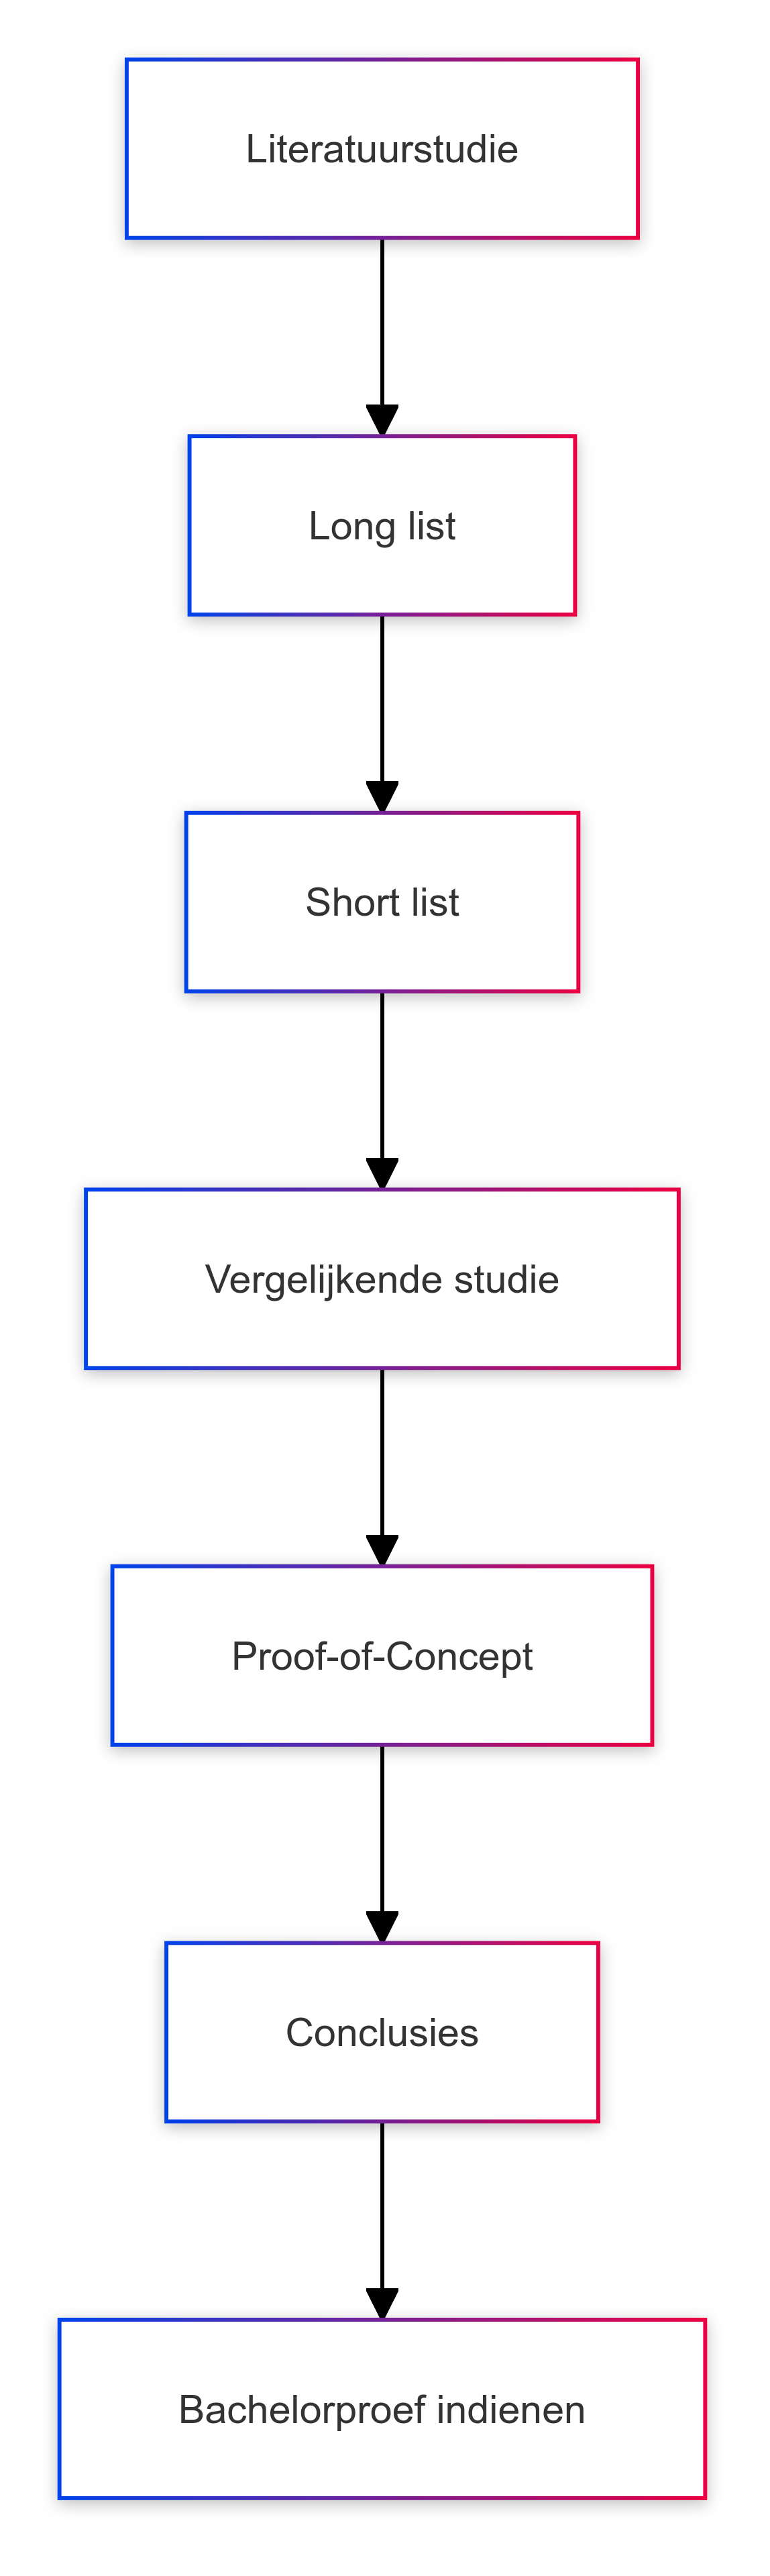
\includegraphics[scale=0.1]{MermaidChart.png}
  \caption{Mermaid flowchart}
  \label{fig:mermaid-chart}
\end{figure}

\begin{figure}[h]
  \centering
  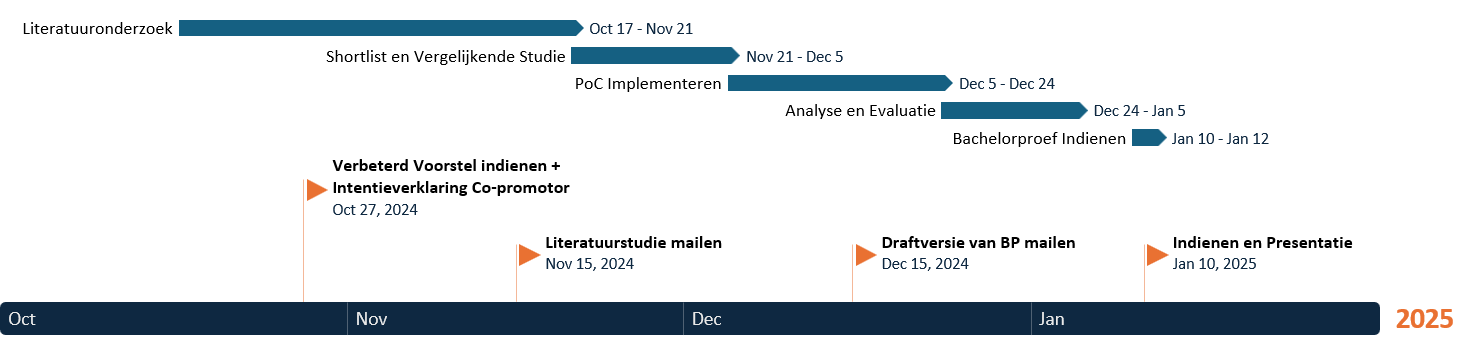
\includegraphics[width=1.0\textwidth]{GanttChart.png}
  \caption{Gantt chart}
  \label{fig:gantt-chart}
\end{figure}

%```mermaid
%flowchart TD
    %A[Indienen verbeterd voorstel] --> B[Bronnen zoeken];
    %B --> C[Bronnen uitschrijven];
    %C --> D[Analyse Methodologie];
    %D --> E[Conclusie Methodologie];
    %E --> F[Bachelorproef herlezen];
    %F --> G[Bachelorproef indienen];
%```
